\section{Optimierung der Empfehlungsqualität}
\label{chap:opt}
% V-Ansatz Teil 3 – Evaluation und Optimierung

% TODO: NDCG@10 Skalen der Abbildungen vereinheitlichen

\subsection{Zielfunktion}
\label{sec:target_function}
Als Zielfunktion für die Optimierung des hybriden Empfehlungssystems dient eine gewichtete 
Linearkombination der Scores der beiden zugrundeliegenden Modelle. Dieser Ansatz wurde 
aufgrund seiner einfachen Interpretierbarkeit und seiner weiten Verbreitung als robuste 
Baseline für hybride Architekturen gewählt (vgl. \cite{burke_hybrid_2002}). 
Die mathematische Formulierung der Funktion lautet:

\begin{equation}
\label{eq:target}
s_\mathrm{hybrid} = w_\mathrm{cbf} \cdot s_\mathrm{cbf} + w_\mathrm{cf} \cdot s_\mathrm{cf}
\end{equation}

Die einzelnen Terme der Gleichung sind wie folgt definiert:
\begin{itemize}
    \item $s_\mathrm{hybrid}$: Der finale, kombinierte Score für ein potenziell zu empfehlendes Item. 
    Die finale Empfehlungsliste wird durch das absteigende Sortieren der Items nach diesem Score erstellt.
    
    \item $s_\mathrm{cbf}$ und $s_\mathrm{cf}$: Die von der Content-Based- bzw. der Collaborative-Filtering-Komponente 
    generierten Roh-Scores. Vor der Kombination in der Zielfunktion ist eine Normalisierung dieser 
    Scores erforderlich, um sicherzustellen, dass sie auf einer vergleichbaren Skala liegen.
    In dieser Arbeit werden die Scores mit der Min-Max-Skalierung auf $[0, 1]$ normalisiert.
    
    \item $w_\mathrm{cbf}$ und $w_\mathrm{cf}$: Die nicht-negativen Gewichtungsparameter, welche den Einfluss 
    der jeweiligen Modellkomponente auf das Endergebnis steuern. Für diese Gewichte gilt die Nebenbedingung 
    $w_\mathrm{cbf} + w_\mathrm{cf} = 1$, wodurch die Optimierung auf die Bestimmung eines einzigen 
    Parameters reduziert wird.
\end{itemize}

Das zentrale Ziel des in~\ref{sec:opt_strat} beschriebenen Optimierungsprozesses 
ist es, die optimalen Werte für die Gewichtungsparameter $w_\mathrm{cbf}$ und $w_\mathrm{cf}$ zu finden, 
sodass die in Abschnitt~\ref{sec:metrics} definierte Evaluationsmetrik (nDCG@10) maximiert wird.

\subsection{Evaluationsmetriken}
\label{sec:metrics}
Die empirische Bewertung und Optimierung des hybriden Empfehlungssystems erfordert ein klar definiertes 
Evaluationsprotokoll sowie eine geeignete Zielfunktion. Als primäre Zielfunktion für die in Kapitel 4 
beschriebene Hyperparameter-Optimierung dient die Maximierung der Empfehlungsqualität, gemessen durch 
den normalisierten diskontierten kumulativen Gewinn bei einer Listenlänge von 10 (nDCG@10). Diese Metrik 
wurde ausgewählt, da sie nicht nur die reine Trefferquote erfasst, sondern vor allem die exakte Position 
eines relevanten Treffers innerhalb der Empfehlungsliste gewichtet, was das reale Nutzerverhalten präzise abbildet.

Die besondere Eignung des nDCG als Metrik für Empfehlungssysteme liegt in seiner positions-sensitiven 
("top-heavy") Natur. Mathematisch wird dies durch eine logarithmische Diskontierung erreicht, bei der der 
Wert eines Treffers am Rang $r$ mit dem Faktor $1/\log_2(r+1)$ abgewertet wird. Dies führt dazu, dass ein 
Treffer an den vordersten Rängen überproportional mehr zur Gesamtbewertung beiträgt als ein Treffer an einer 
späteren Position. So ist beispielsweise ein relevanter Artikel an Rang 1 signifikant wertvoller als 
an Rang 2, während der Unterschied zwischen Rang 100 und 101 nur noch marginal ist. Diese Eigenschaft ist 
essenziell, da Nutzer Interaktionen auf den vordersten Plätzen der Ergebnisliste konzentrieren und weiter 
hinten platzierte Vorschläge selten beachten (vgl. \cite{krichene_sampled_2020}).

Ein entscheidender Aspekt des Evaluationsdesigns ist die Handhabung negativer Instanzen. Anstatt auf 
Verfahren des Negative Samplings zurückzugreifen, bei denen eine kleine, zufällige Teilmenge 
nicht-interagierter Artikel als negative Beispiele dient, wird in dieser Arbeit eine 
methodisch rigorosere Strategie des \textit{Full-Catalog Rankings} verfolgt. Bei diesem Vorgehen muss 
das Modell für jeden positiven Testfall den relevanten Artikel aus der Gesamtheit aller im 
Datensatz verfügbaren Artikel – abzüglich der bereits vom Nutzer gelesenen – identifizieren.

Diese Methode vermeidet systematische Verzerrungen (sampling bias), die durch ein 
unausgewogenes Sampling entstehen können, und simuliert ein anspruchsvolles, aber realistisches 
Anwendungsszenario. Die Evaluation auf dem gesamten Artikelkatalog stellt eine enorme 
Herausforderung für das Empfehlungssystem dar, was naturgemäß zu absolut gesehen niedrigen 
Metrikwerten führt. Wie in der Fachliteratur bestätigt wird, sind solche Ergebnisse jedoch nicht 
als Indikator für eine geringe Modellleistung zu interpretieren, sondern als Konsequenz eines 
besonders anspruchsvollen und unverzerrten Evaluationsprotokolls 
(vgl. \cite{krichene_sampled_2020}). Die auf diese Weise gewonnenen Erkenntnisse bieten eine 
robuste und verlässliche Grundlage für die zukünftige Weiterentwicklung von 
Empfehlungssystemen bei der SV-Gruppe.

\subsection{Experimenteller Aufbau und Validierungsdatensatz}
Die Grundlage für die Optimierung und Evaluation bildet ein Validierungsdatensatz, der aus den 
Nutzerinteraktionen der letzten Januarwoche 2025 extrahiert wurde. Die statistischen Kennzahlen 
dieses Zeitraums sind in Tabelle~\ref{tab:statistiken_test} zusammengefasst.

% content/tables/statistiken_testdaten.tex

\begin{table}[htbp]
    \centering
    \caption{Statistische Kennzahlen des Test- und Validierungsdatensatzes, basierend auf den Klick-Logs der letzten Januarwoche.}
    \label{tab:statistiken_test}
    \begin{tabular}{lr}
        \toprule
        \textbf{Metrik} & \textbf{Wert} \\
        \midrule
        Gesamte Artikelaufrufe & 3.627.024 \\
        Einzigartige user\_pseudo\_ids & 1.099.289 \\
        Einzigartige Artikel & 57.100 \\
        \bottomrule
    \end{tabular}
\end{table}

Aus dem Gesamt-Pool an Nutzern wurde eine repräsentative Validierungsstichprobe von 1.000 
einzigartigen Nutzern zufällig gezogen, um den für die Optimierung erforderlichen Rechenaufwand in einem praktikablen 
Rahmen zu halten. Für jeden Nutzer in der Stichprobe wurde nach dem \textit{Leave-Last-Out}-Prinzip 
der letzte interagierte Artikel als Ground Truth für die Evaluation definiert (vgl. \Cite{Rendle_BPR_2009}).

\subsection{Optimierungsstrategie}
\label{sec:opt_strat}
Die Bestimmung der optimalen Gewichtungsparameter $w_\mathrm{cbf}$ und $w_\mathrm{cf}$ aus 
Gleichung~\ref{eq:target} erfolgt durch einen automatisierten Hyperparameter-Optimierungsprozess.

Als Framework für diesen Prozess wurde \textit{Optuna} (\Cite{Akiba_Optuna_2019}) gewählt, das eine effiziente Suche im 
Parameterraum ermöglicht. Über insgesamt 515 Iterationen (Trials) wurden verschiedene 
Gewichtungskombinationen evaluiert, mit dem Ziel, die in Abschnitt~\ref{sec:metrics} definierte 
nDCG@10-Metrik zu maximieren.

Der Ablauf eines einzelnen Optimierungs-Trials gestaltet sich wie folgt:
\begin{enumerate}
    \item Optuna schlägt eine neue Wertekombination für $w_\mathrm{cbf}$ und $w_\mathrm{cf}$ vor.
    \item Für jeden der 1.000 Nutzer in der Validierungsstichprobe werden die Empfehlungen der 
    \ac{CBF}- und \ac{CF}-Modelle über deren jeweilige API-Endpunkte parallel und asynchron abgerufen.
    \item Die Ergebnislisten der beiden Modelle werden mittels der vorgeschlagenen Gewichte zu einer 
    finalen hybriden Empfehlungsliste fusioniert.
    \item Der nDCG@10-Wert dieser finalen Liste wird berechnet, indem sie mit dem Ground-Truth-Artikel 
    des Nutzers verglichen wird.
    \item Der über alle 1.000 Nutzer gemittelte nDCG@10-Wert wird an Optuna zurückgegeben, um 
    den nächsten, informierteren Suchschritt zu steuern.
\end{enumerate}

Dieser Prozess entspricht einem Gesamtaufwand von 515.000 individuellen Evaluierungen des 
Hybridmodells, was eine gründliche und robuste Suche nach der optimalen Parameterkonfiguration 
gewährleistet.

Die Visualisierung der Optimierungslandschaft in Abbildung~\ref{fig:hyperparameterraum} verdeutlicht die 
komplexe, nicht-lineare Beziehung zwischen den Modellgewichten und der resultierenden Empfehlungsqualität. 
Angesichts dieser zerklüfteten Landschaft mit mehreren lokalen Optima ist ein naiver Ansatz wie eine 
Rastersuche (Grid Search) ineffizient. Der Einsatz eines fortschrittlichen Optimierungsframeworks 
wie Optuna, das mit intelligenten Suchalgorithmen arbeitet, ist daher notwendig, um den global 
optimalen Bereich im Parameterraum effizient und verlässlich zu identifizieren.

% content/figures/plot_hyperparameterraum.tex

\begin{figure}[H]
    \centering
    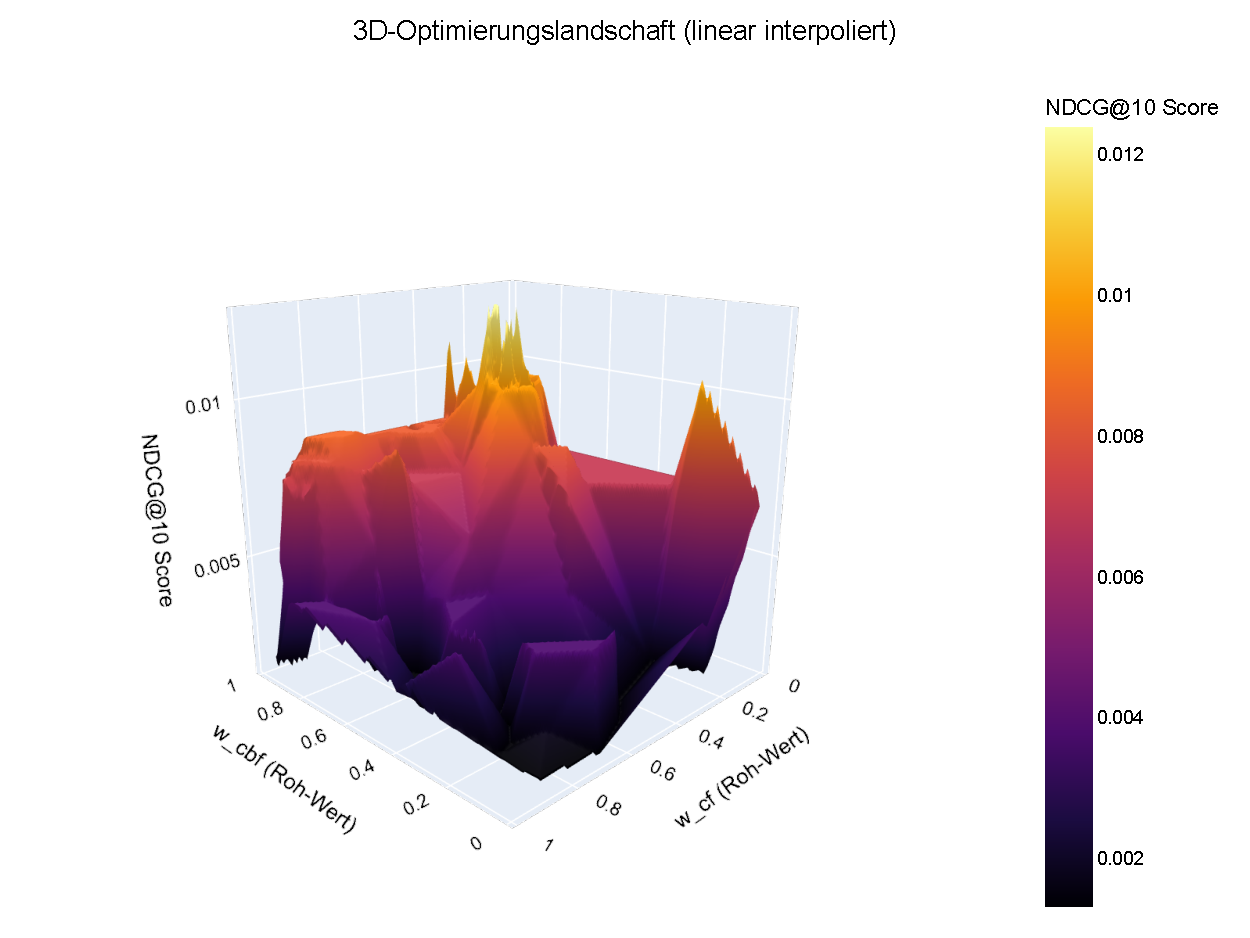
\includegraphics[width=0.9\textwidth]{content/figures/svg/hyperparameterraum.pdf}
    \caption{Visualisierung des zweidimensionalen Hyperparameterraums der Modellgewichtungen. Die Achsen repräsentieren die Gewichte für das CBF-Modell (\(w_{cbf}\)) und das CF-Modell (\(w_{cf}\)). Die Einfärbung der Punkte visualisiert den resultierenden NDCG@10-Wert für jede Konfiguration aus dem Optuna-Suchlauf.}
    \label{fig:hyperparameterraum}
\end{figure}

Konkret wurde für die Suche der in Optuna standardmäßig implementierte \ac{TPE} als Suchalgorithmus verwendet (vgl. \cite{Akiba_Optuna_2019}). Der TPE-Algorithmus ist eine 
Variante der Bayes'schen Optimierung, die ein probabilistisches Modell der Zielfunktion erstellt, 
um intelligent zu entscheiden, welche Parameterkombination als Nächstes getestet werden soll. 
Dafür werden die bisherigen Evaluationsergebnisse in eine Gruppe mit vielversprechenden
und eine mit weniger erfolgreichen Ergebnissen aufgeteilt.

Für beide Gruppen werden separate Wahrscheinlichkeitsverteilungen modelliert. Der Algorithmus maximiert 
anschließend die erwartete Verbesserung Expected Improvement, indem er gezielt nach Parametern sucht, 
die eine hohe Wahrscheinlichkeit unter der Verteilung der guten Ergebnisse und gleichzeitig eine 
niedrige Wahrscheinlichkeit unter der Verteilung der schlechten Ergebnisse aufweisen. Diese Strategie 
ermöglicht eine effiziente Balance zwischen der Exploitation bereits bekannter guter 
Regionen und der Exploration neuer, potenziell noch besserer Bereiche des Suchraums. 
Durch diesen informierten Suchprozess kann das Optimum in komplexen Landschaften, wie der in 
Abbildung~\ref{fig:hyperparameterraum} gezeigten, deutlich schneller und ressourcenschonender 
gefunden werden als durch uninformierte Methoden.

\subsection{Ergebnisse}
\label{sec:results}
Der in Abschnitt~\ref{sec:opt_strat} beschriebene Optimierungsprozess führte zur Identifikation 
einer robusten Gewichtungskonfiguration für das hybride Empfehlungssystem. Die finale 
Evaluation zeigt, dass das optimierte Hybrid-Modell die definierten Baseline-Modelle 
in allen Metriken signifikant übertrifft.

Tabelle~\ref{tab:baseline_vergleich} listet die detaillierten Performance-Werte der evaluierten 
Modellvarianten auf, während Abbildung~\ref{fig:model_vergleich} eine visuelle 
Gegenüberstellung der Ergebnisse bietet.

% Inhalt von: content/tables/vergleich_baselines.tex

\begin{table}[htbp]
    \centering
    \caption{Vergleich des optimierten Hybrid-Modells mit den Baseline-Modellen anhand der Metriken NDCG@10 und Hit Rate@10.}
    \label{tab:baseline_vergleich}
    \begin{tabular}{lrr}
        \toprule
        \textbf{Modell} & \textbf{NDCG@10} & \textbf{Hit Rate@10} \\
        \midrule
        Unser Hybrid-Modell (Final) & 1.25\% & 1.8\% \\
        Popularity-Baseline        & 0.23\% & 0.6\% \\
        Recency-Baseline           & 0.14\% & 0.4\% \\
        \bottomrule
    \end{tabular}
\end{table}

% content/figures/vergleich_baselines.tex

\begin{figure}[H]
    \centering
    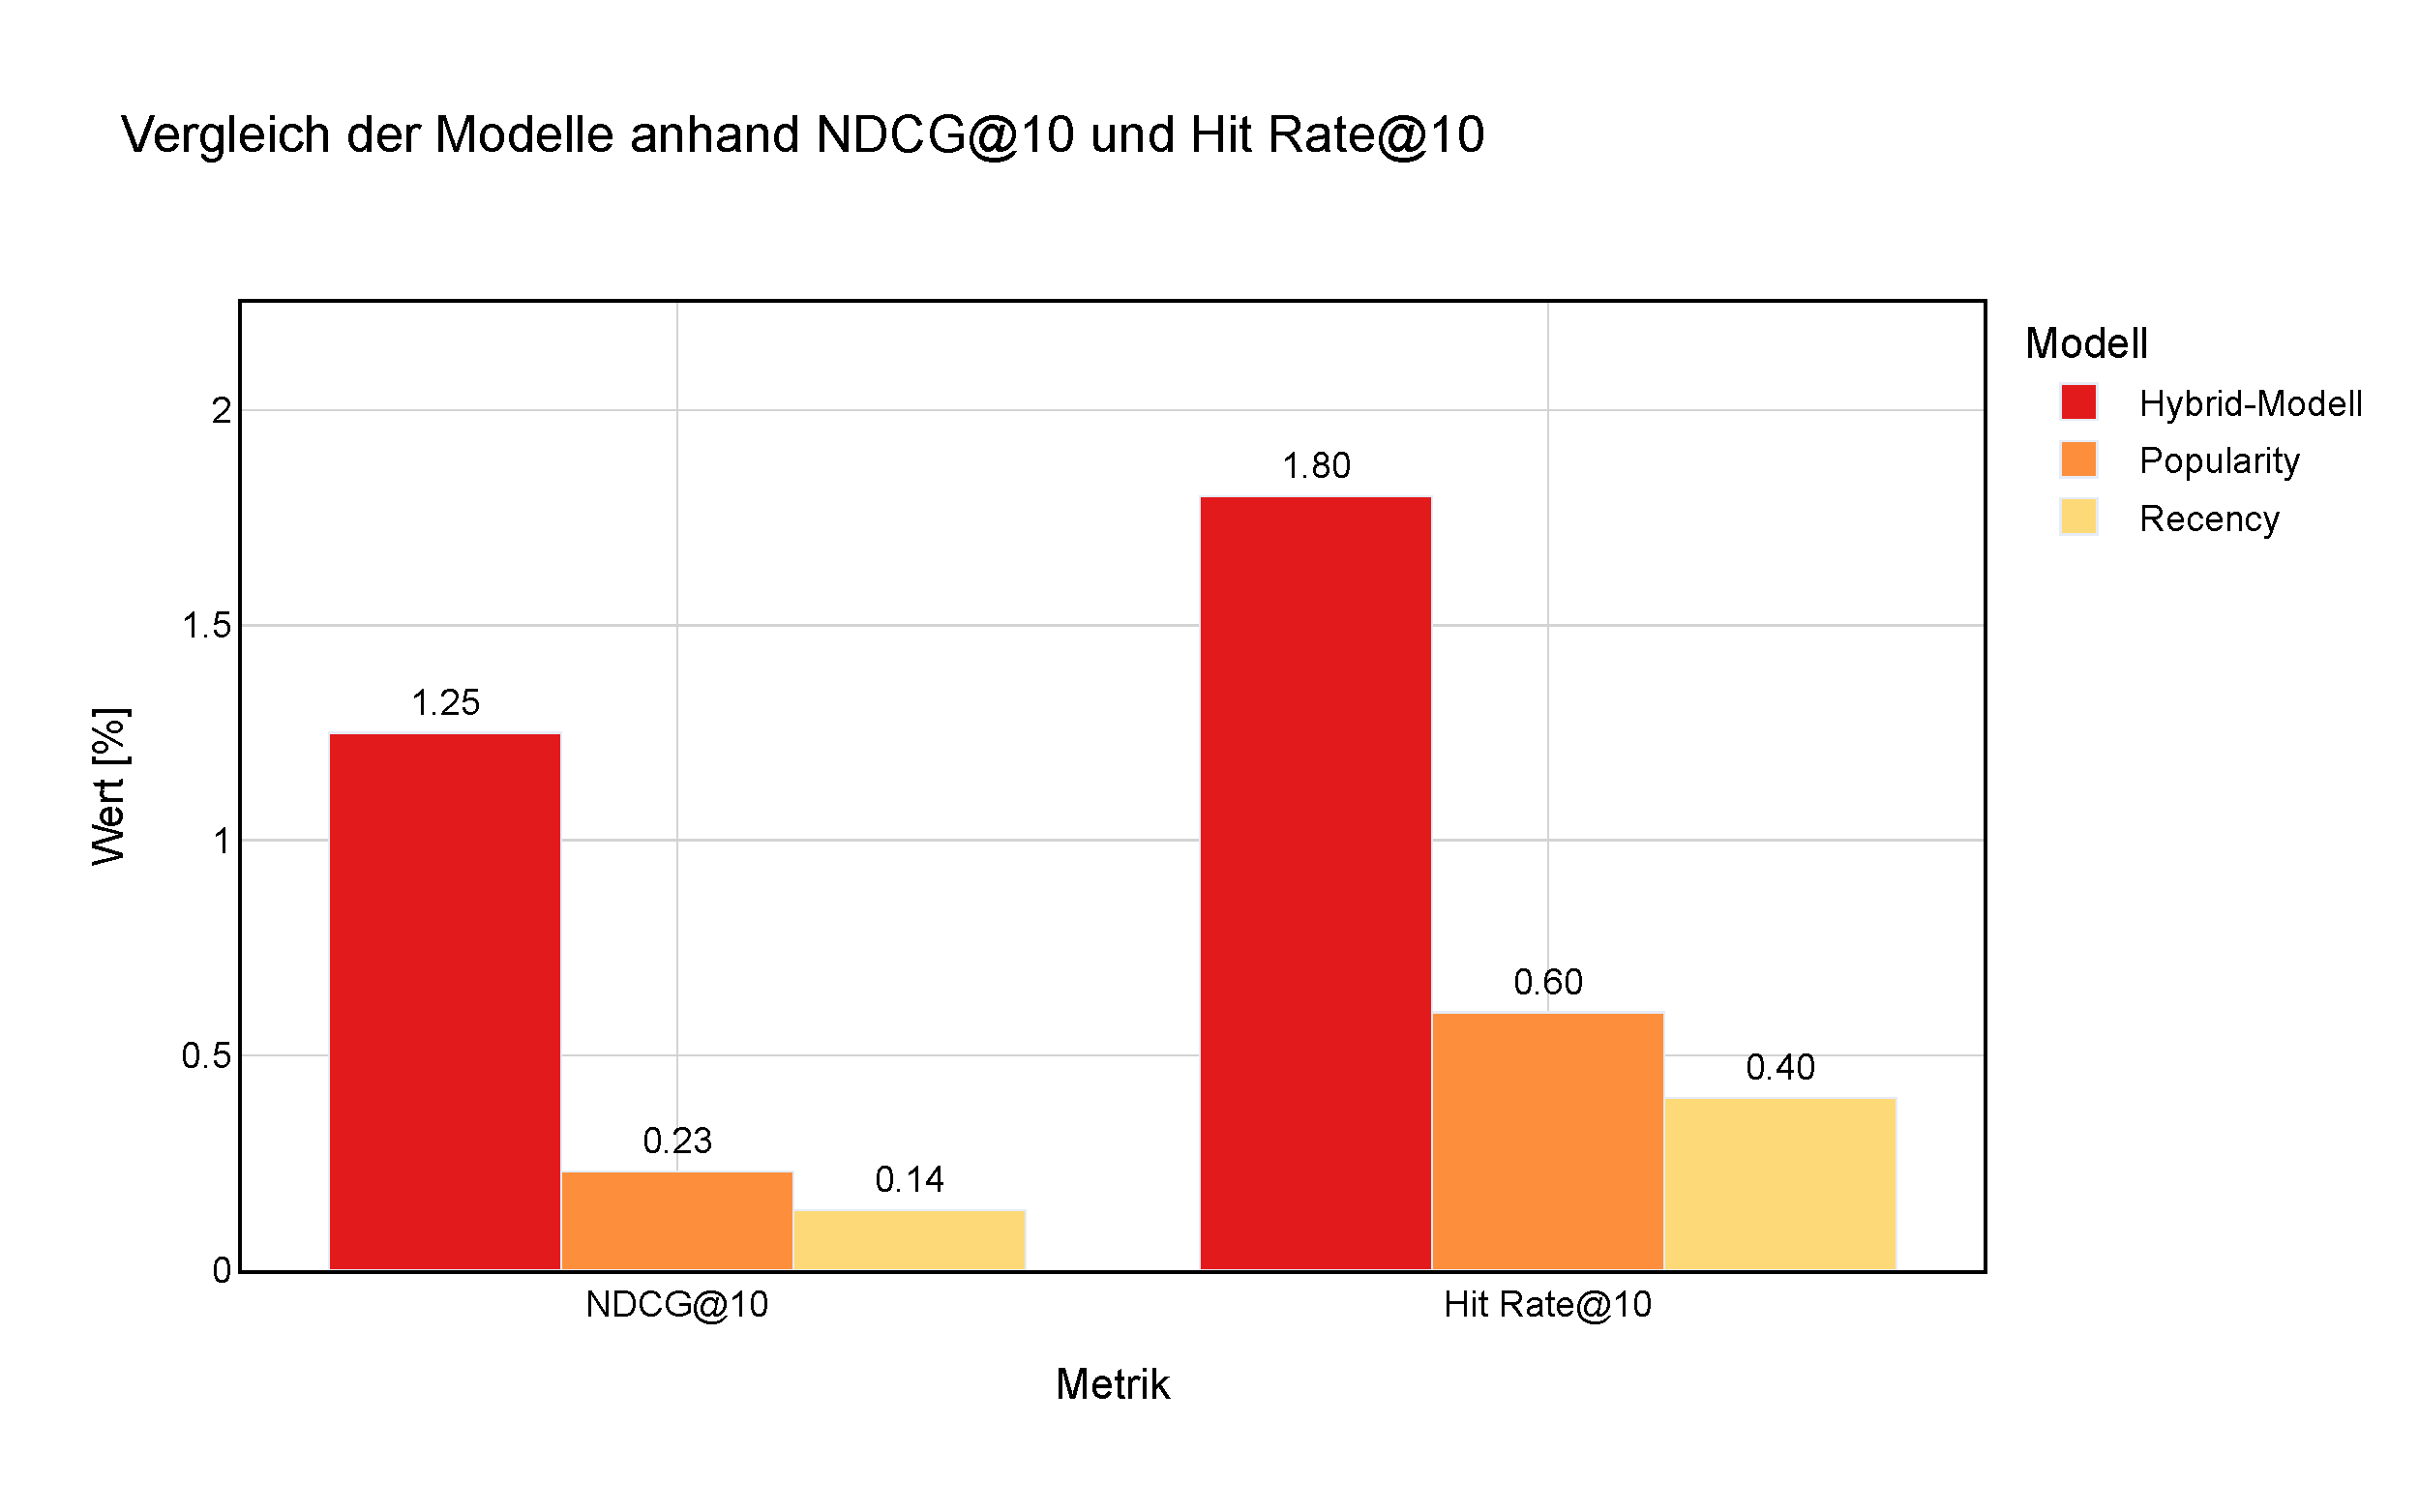
\includegraphics[width=0.8\textwidth]{content/figures/svg/model_baseline_comparison.pdf}
    \caption{Vergleich des Hybrid-Modells mit den Popularity- und Recency-Baselines anhand der Metriken NDCG@10 und Hit Rate@10.}
    \label{fig:model_vergleich}
\end{figure}

Abbildung~\ref{fig:kontourplot} zeigt die einzelnen Trials (Schwarze Punkte) auf der Hyperparameterlandschaft. 
Es ist gut zu erkennen, dass die größte Anzahl an optima in einem Bereich liegt, in dem $w_{cbf}$ größer als 0.5 ist und
$w_{cf}$ kleiner als 0.5.

Diese Ergebnisse bestätigen nicht nur die Wirksamkeit des gwählten
Hybridisierungsansatzes, sondern liefern auch den empirischen Beleg für dessen Überlegenheit gegenüber den reinen
Einzelkomponenten. Der Optimierungsprozess durchsuchte den gesamten Gewichtungsraum, einschließlich der Extremfälle,
die einem reinen \ac{CF}-Modell ($w_{cf} = 1$) oder einem reinen \ac{CBF}-Modell ($w_{cb} = 1$) entsprechen.
% content/figures/plot_kontour.tex

\begin{figure}[htbp]
    \centering
    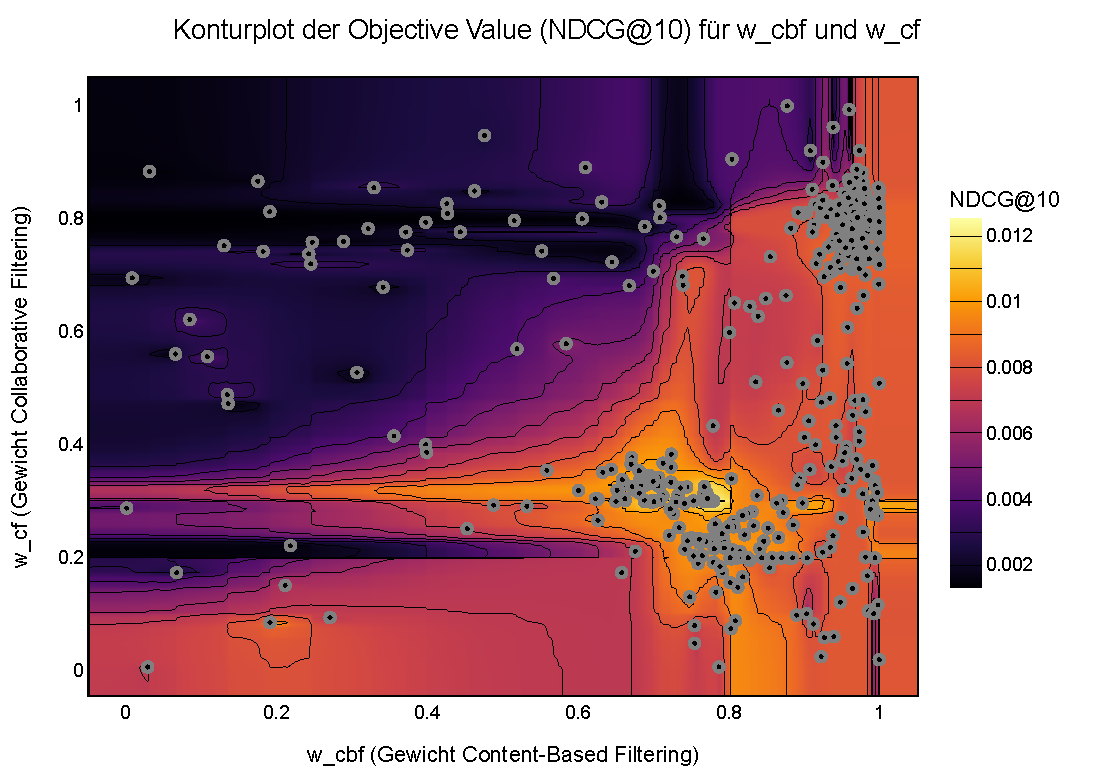
\includegraphics[width=0.9\textwidth]{content/figures/svg/kontourplot.pdf}
    \caption{Konturplot zur Darstellung der NDCG@10-Verteilung im zweidimensionalen Parameterraum der Modellgewichtungen. Die Isolinien verbinden Bereiche mit ähnlicher Performance.}
    \label{fig:kontourplot}
\end{figure}
Das identifizierte Optimum liegt jedoch klar bei einer Konfiguration von \(w_{cbf} \approx 0.7226\) und
\(w_{cf} \approx 0.2774\). Diese Tatsache belegt, dass beide Komponenten einen positiven Beitrag zur Maximierung
des \ac{nDCG}@10 leisten und die gewichtete Kombination eine signifikant höhere Empfehlungsqualität erzielt, als es durch den
alleinigen Einsatz des \ac{CBF}- oder \ac{CF}-Modells möglich gewesen wäre. Die konzeptionelle Notwendigkeit des hybriden
Ansatzes zur Ausbalancierung von Relevanz und Diversität wird somit durch die datengetriebene Optimierung quantitativ
untermauert.

Die dominante Rolle der \ac{CBF}-Komponente wird in Abbildung~\ref{fig:2d_performance} nochmals verdeutlicht. Die 
Visualisierung zeigt die \ac{nDCG}@10 Performance aller 515 Trialsin Abhängigkeit vom normalisierten \ac{CBF}-Gewicht.

Es ist ein deutlicher Leistungssprung (Phasensprung) bei einem Gewicht von \(w_{cbf} \approx 0.5\) zu erkennen.
Unterhalb dieser Schwelle werden durchweg nur niedrige \ac{nDCG}@10-Werte erreicht. Oberhalb davon steigt die Performance 
signifikant an, und alle optimalen Ergebnisse (orange markiert) konzentrieren sich im Bereich \(w_{cbf} > 0.6\)

Diese Beobachtung untermauert die Hypothese, dass im Nachrichtenkontext der unmittelbare thematische Bezug zum 
gerade gelesenen Artikel der stärkste Prädiktor für die nächste Interaktion ist. 
Das CBF-Modell liefert hier das notwendige Fundament für eine relevante Empfehlung. 
Die CF-Komponente dient in diesem Zusammenspiel als entscheidender „Fein-Tuner”, der auf dieser starken Basis aufsetzt, 
um die Performance durch Personalisierung auf das globale Maximum zu heben, wie es im Konturplot (Abbildung~\ref{fig:kontourplot}) 
ersichtlich wurde.

% content/figures/plot_2d_performance.tex

\begin{figure}[H]
    \centering
    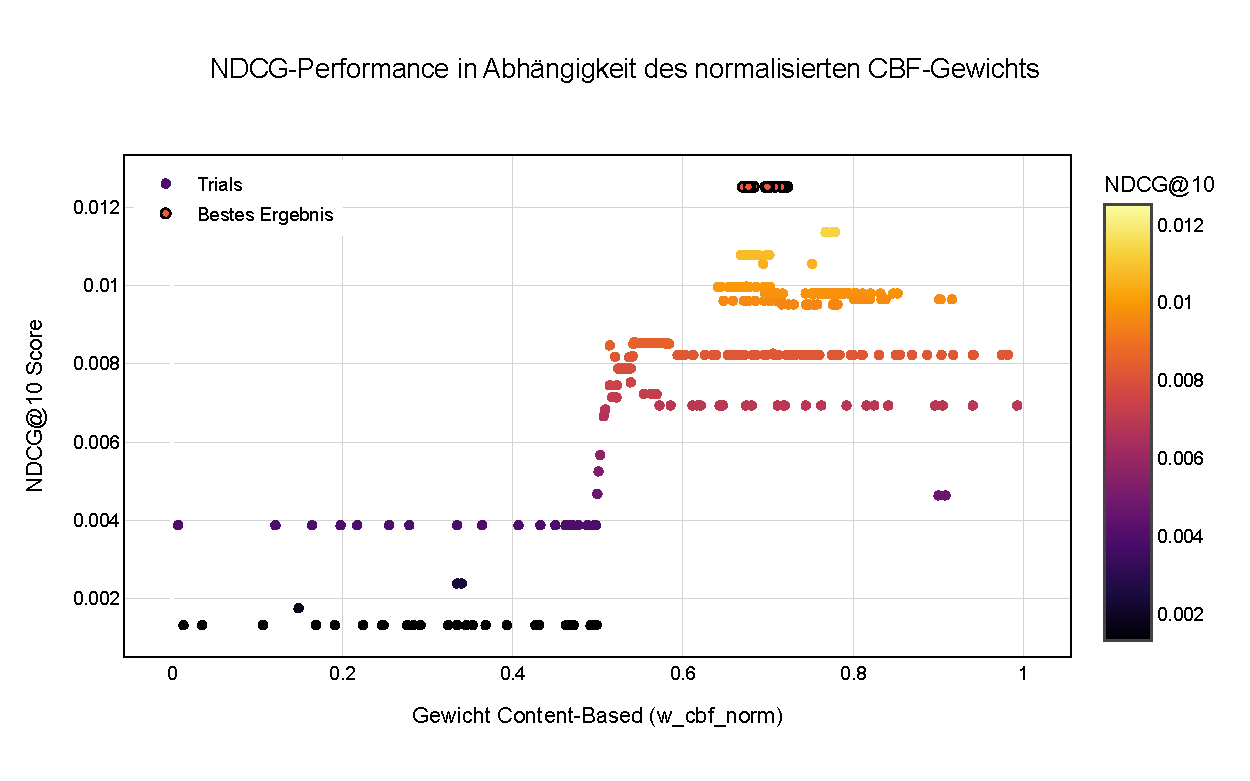
\includegraphics[width=0.9\textwidth]{content/figures/svg/2d_performance.pdf}
    \caption{2D-Darstellung des Hyperparameterraums. Die Achsen zeigen die Gewichtungen für das CBF- (\(w_{cbf}\)) und CF-Modell (\(w_{cf}\)). Die Farbe der Punkte indiziert den erreichten NDCG@10-Score. Der optimale Punkt ist markiert.}
    \label{fig:2d_performance}
\end{figure}
% % content/figures/plot_3d_scatter.tex

\begin{figure}[htbp]
    \centering
    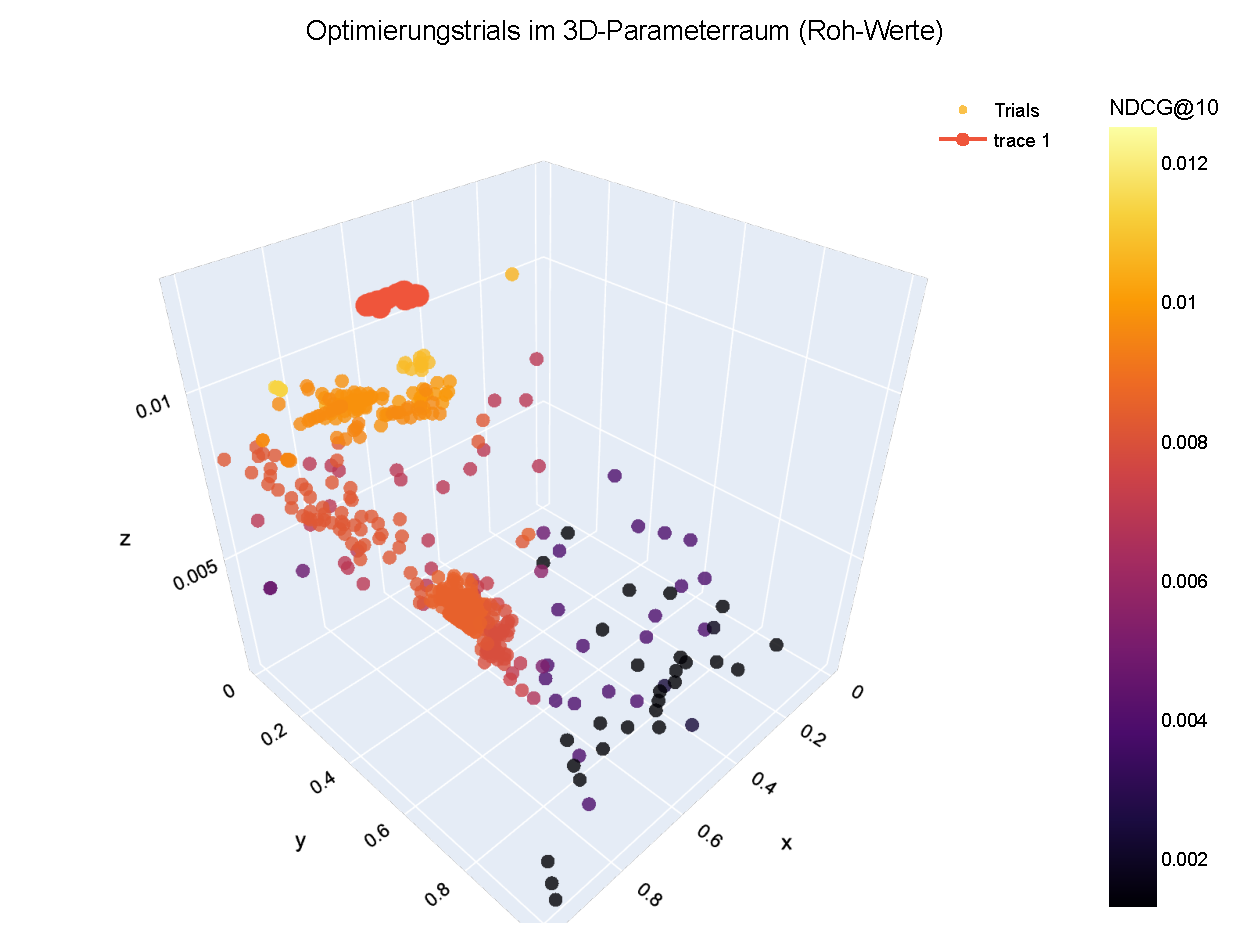
\includegraphics[width=0.8\textwidth]{content/figures/svg/3d_scatter_plot.pdf}
    \caption{Interaktives 3D-Streudiagramm der Optuna-Trials zur Visualisierung der Parameterabhängigkeiten. (Hinweis: Die Darstellung in der PDF-Version der Arbeit ist eine statische Ansicht).}
    \label{fig:3d_scatter}
\end{figure}